\documentclass[a4paper,12pt,francais,twoside]{article}

\input{../style/imports}

\SetInfo
{
  annee-universitaire = 2015-2016,
  grade               = Master 1,
  mention             = MIAGE,
  responsable        = {L.M. Hillah, P. Poizat},
  EC                  = POO,
  code-APOGEE         = EMIPO119,
  UFR                 = SEGMI,
  etablissement       = Université Paris Ouest Nanterre,
}

\begin{document}

\graphicspath{{../images/}}

\TitreFeuille{Airline Management System}

\input{../style/entete}


\section{Objectif}

L'objectif de ce devoir est de mettre en oeuvre les bonnes pratiques et patrons de conceptions
en programmation orientée-objet. Il s'agit de réaliser une application de gestion de système de gestion aéroportuaire, dont le comportement global est réparti dans un ensemble de classes,
présentées dans la figure~\ref{fig:ams}.

L'application doit permettre à un client de créer des aéroports, des 
compagnies aériennes ainsi que des vols. Le point d'entrée de l'application
est le \texttt{SystemManager}. Chaque compagnie \texttt{Airline} est associé
à  un ensemble de vols (\texttt{Flights}). Un vol a un aéroport de départ 
(\texttt{origin}) et un aéroport d'arrivée (\texttt{destination}). 
L'origine et la destination ne peuvent être les mêmes. 

Chaque vol comprend des classes tarifaires (e.g., première classe, business)
appelées \texttt{flight section}. Chaque classe tarifaire comprend des 
sièges organisés en rangs (ligne et colonne).

\subsection{Consigne}
Vous devez faire fonctionner votre application sur le jeu minimal d'instructions
fourni dans le programme principal à la fin de ce document. 
Vous devez également utiliser un framework de test (JUnit, TestNG), pour 
fournir des jeux de test pour les fonctions critiques de l'application que vous identifierez
et dont vous justifierez le caractère critique (pas de tests sur les getters/setters !).


\begin{figure}[h!]
	\centering
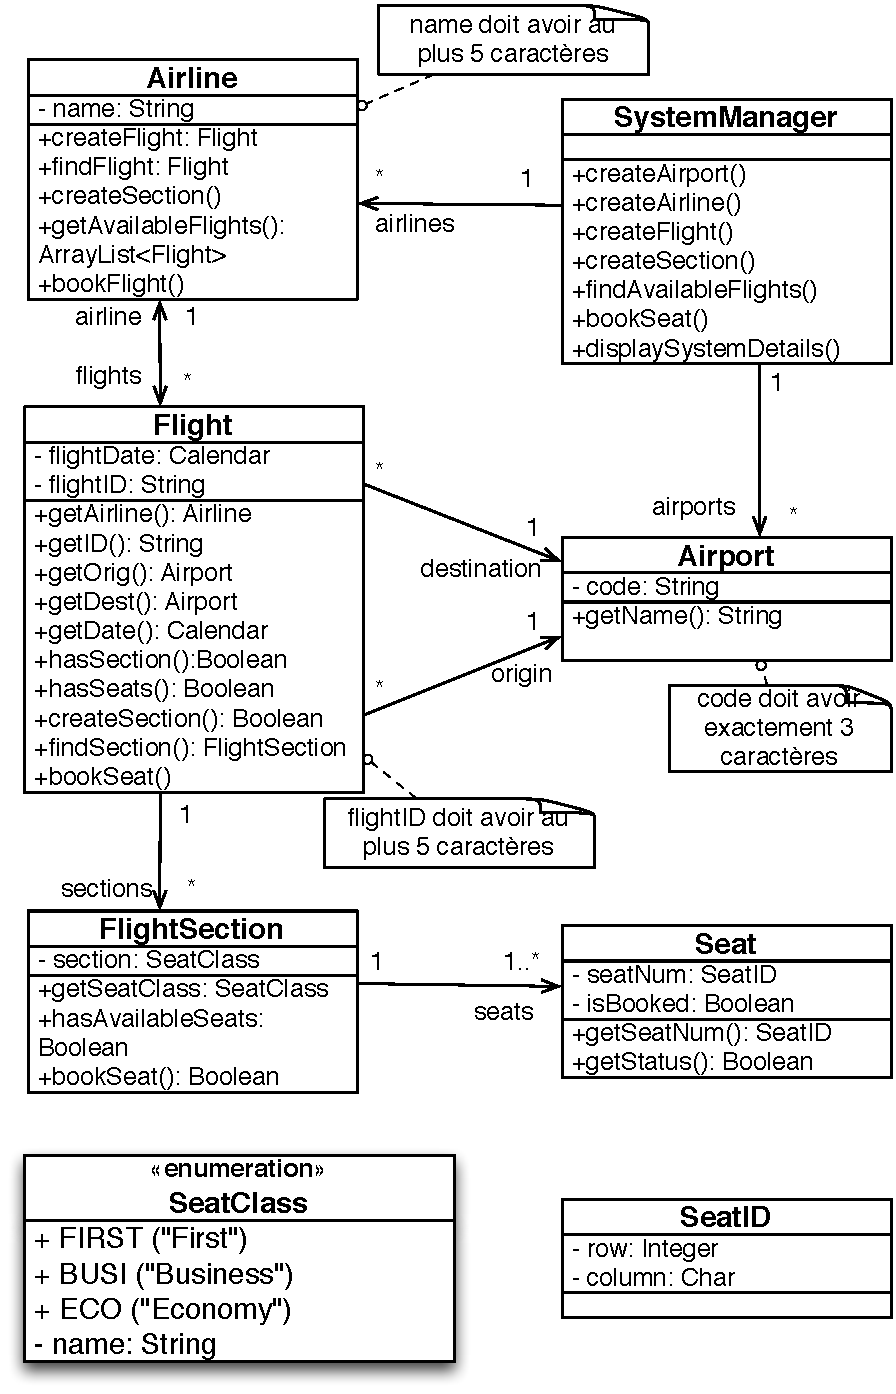
\includegraphics[scale=0.8]{ams}
\caption{Description architecturale de Airline Management System}
\label{fig:ams}
\end{figure}

\section{SystemManager}

C'est le point d'entrée de l'application. Les clients interagissent
avec l'application en appelant les opérations offertes par \texttt{SystemManager}.
Ce dernier est relié aux aéroports et compagnies aériennes dans l'application.
A sa création, le \texttt{SystemManager} ne possède aucun aéroport ou compagnie aérienne.
Pour les créer les opérations \texttt{createAirport()} et \texttt{createAirline()}
doivent être invoquées. 

Le \texttt{SystemManager} contient également les opérations pour créer les
classes tarifaires, trouver les vols disponibles entre deux aéroports, et
réserver des sièges sur un vol. Pour afficher toute l'information concernant
les aéroports les compagnies et les vols, classes tarifaires et sièges, on 
invoque l'opération \texttt{displaySystemDetails()}.

\begin{itemize}
	\item \texttt{createAirport(String n)} : crée un objet de type \texttt{Airport}
	et le lie au \texttt{SystemManager}. L'aéroport doit avoir un code n, dont
	la longueur est exactement égale à 3. Deux aéroports différents ne peuvent avoir le même code.
	\item \texttt{createAirline(String n)} : crée une compagnie aérienne et la lie
	au \texttt{SystemManager}. Le nom n d'une compagnie doit être de longueur au plus
	égale à 5. Deux compagnies différentes ne peuvent avoir le même nom.
	\item \texttt{createFlight(String n, String orig, String dest, int year, int month, int day, String id)} : crée un vol pour une compagnie n, en invoquant l'opération \texttt{createFlight} sur
	la classe \texttt{Airline}.
	\item \texttt{createSection(String air, String flID, int rows, int cols, SeatClass s)} : crée
	une section tarifaire, de classe s, pour un vol identifié par flID, associé à une compagnie
	air, en invoquant l'opération \texttt{createSection()} de la classe \texttt{Airline}.
	La section contiendra le nombre de lignes et de colonnes.
	\item \texttt{findAvailableFlights(String orig, Strin dest)} : trouve tous les vols
	pour lesquels il existe encore des sièges disponibles, entre les aéroports
	de départ et d'arrivée.
	\item \texttt{bookSeat(String air, String fl, SeatClass s, int row, char col)} : 
	réserve le siège dont la position est indiquée par row et col (e.g. 15A), sur le
	vol fl de la compagnie air.
	\item \texttt{displaySystemDetails()} : affiche toute l'information concernant
	tous les objets (e.g. aéroports, compagnies, vols, sièges, ...) dans le système.
\end{itemize}


\section{Airport}
Un objet de cette classe représente un aéroport. Il possède un nom, de longueur 3 caractères.

\section{Airline}
Cette classe définit une compagnie aérienne. Une compagnie possède zéro ou plusieurs
vols en cours. A la création d'un objet de ce type, il n'y a initialement aucun vol.
Chaque vol doit avoir un identifiant unique.

\begin{itemize}
	\item \texttt{Flight createFlight(String orig, String dest, Calendar date, String id)} : crée
	un vol pour une compagnie aérienne.
	\item \texttt{Flight findFlight(String n)} : trouve un vol dont l'identifiant est n.
	\item \texttt{createSection(String flID, int rows, int cols, SeatClass s)} : crée une section
	tarifaire de classe s, pour un vol dont l'identifiant est flID. La section contiendra le
	nombre de lignes et de colonnes.
	\item \texttt{ArrayList<Flight> getAvailableFlights(Airport orig, Airport dest)} : trouve tous les
	vols sur lesquels il existe encore des sièges disponibles, entre les aéroports de départ
	et d'arrivée.
	\item \texttt{bookFlight(String fl, SeatClass s, int row, char col)} : réserve un siège dont
	la position est indiquée par row et col (e.g. 15A) dans la section tarifaire s, sur le vol fl.
\end{itemize}

\section{FlightSection}
Cette classe définit une classe (ou section) tarifaire. Chaque section possède une classe
(première, affaires, ou économique) et au moins 1 siège.  Une FlightSection possède 
des attributs nombre de rows et nombre de columns, afin de savoir combien de sièges elle contient
et le calcul du nombre de sièges disponibles.

Une section tarifaire contient au plus 100 rangées de sièges et au plus 10 sièges par rangée.

\begin{itemize}
	\item \texttt{hasAvailableSeats()}
	renvoie vrai si et seulement si la section possède encore des sièges disponibles (non réservés).
	\item \texttt{bookSeat()} réserver le premier siège disponible. Son utilisation est conditionnée
	à celle de \texttt{hasAvailableSeats()}.
	\item \texttt{boolean bookSeat(SeatID sId)} réserver le siège à l'emplacement désigné par le
	paramètre sID, si ce siège est disponible.
\end{itemize}


\section{Seat}
Cette classe définit un siège. Un siège possède un identificateur, qui indique sa rangée
et sa colonne (caractère allant de A à J). Il possède également un statut qui indique 
s'il est réservé ou pas.

\section{Client de l'application}
Un exemple de client de cette application est fourni dans la classe \texttt{ClientAMS}.
Ce client appelle des opérations de la classe \texttt{SystemManager}.

Vous êtes invités à étendre cette classe client avec d'autres invocations pour
tester le comportement attendu de votre application.

\begin{lstlisting}
public class ClientAMS {
    public static void main (String[] args) {
        SystemManager res = new SystemManager();
		// Airports
		res.createAirport("DEN");
		res.createAirport("DFW");
		res.createAirport("LON");
		res.createAirport("DEN");
		res.createAirport("CDG");
		res.createAirport("JPN");
		res.createAirport("DEN"); // Pb d'unicite
		res.createAirport("DE"); // Invalide
		res.createAirport("DEH");
		res.createAirport("DRIrdn3"); // Invalide
		
		// Airlines
		res.createAirline("DELTA");
		res.createAirline("AIRFR");
		res.createAirline("AMER");
		res.createAirline("JET");
		res.createAirline("DELTA");
		res.createAirline("SWEST");
		res.createAirline("FRONTIER");  // Invalide
		
		// Flights
		res.createFlight("DELTA", "DEN", "LON", 2008, 11, 12, "123");
		res.createFlight("DELTA", "DEN", "DEH", 2009, 8, 9, "567");
		res.createFlight("DELTA", "DEN", "NCE", 2010, 9, 8, "567"); // Invalide
		
		// Sections
		res.createSection("JET", "123", 2, 2, SeatClass.economy);
		res.createSection("JET", "123", 1, 3, SeatClass.economy);
		res.createSection("JET", "123", 2, 3, SeatClass.first);
		res.createSection("DELTA", "123", 1, 1, SeatClass.business);
		res.createSection("DELTA", "123", 1, 2, SeatClass.economy);
		res.createSection("SWSERTT", "123", 5, 5, SeatClass.economy); // Invalide
		
		res.displaySystemDetails();
		
		res.findAvailableFlights("DEN", "LON");
		
		res.bookSeat("DELTA", "123", SeatClass.business, 1, 'A');
		res.bookSeat("DELTA", "123", SeatClass.economy, 1, 'A');
		res.bookSeat("DELTA", "123", SeatClass.economy, 1, 'B');
		res.bookSeat("DELTA", "123", SeatClass.business, 1, 'A'); // Deja reserve
		
		res.displaySystemDetails();
		
		res.findAvailableFlights("DEN", "LON");
    }
}
\end{lstlisting}

\end{document}
